\documentclass[a4paper,12pt]{article}

\usepackage[utf8]{inputenc}
\usepackage{amsmath, amssymb}
\usepackage{graphicx}
\usepackage{hyperref}
\usepackage{pdfpages}
\usepackage{enumitem}
\usepackage{array}

\title{Pretest Practice}
\author{Niccolò Gabrielli}
\date{\today}

\newcolumntype{C}[1]{>{\centering\arraybackslash}m{#1}}  % Centered m-column






\begin{document}

\maketitle

\tableofcontents
\newpage


\section{24-01-2025}

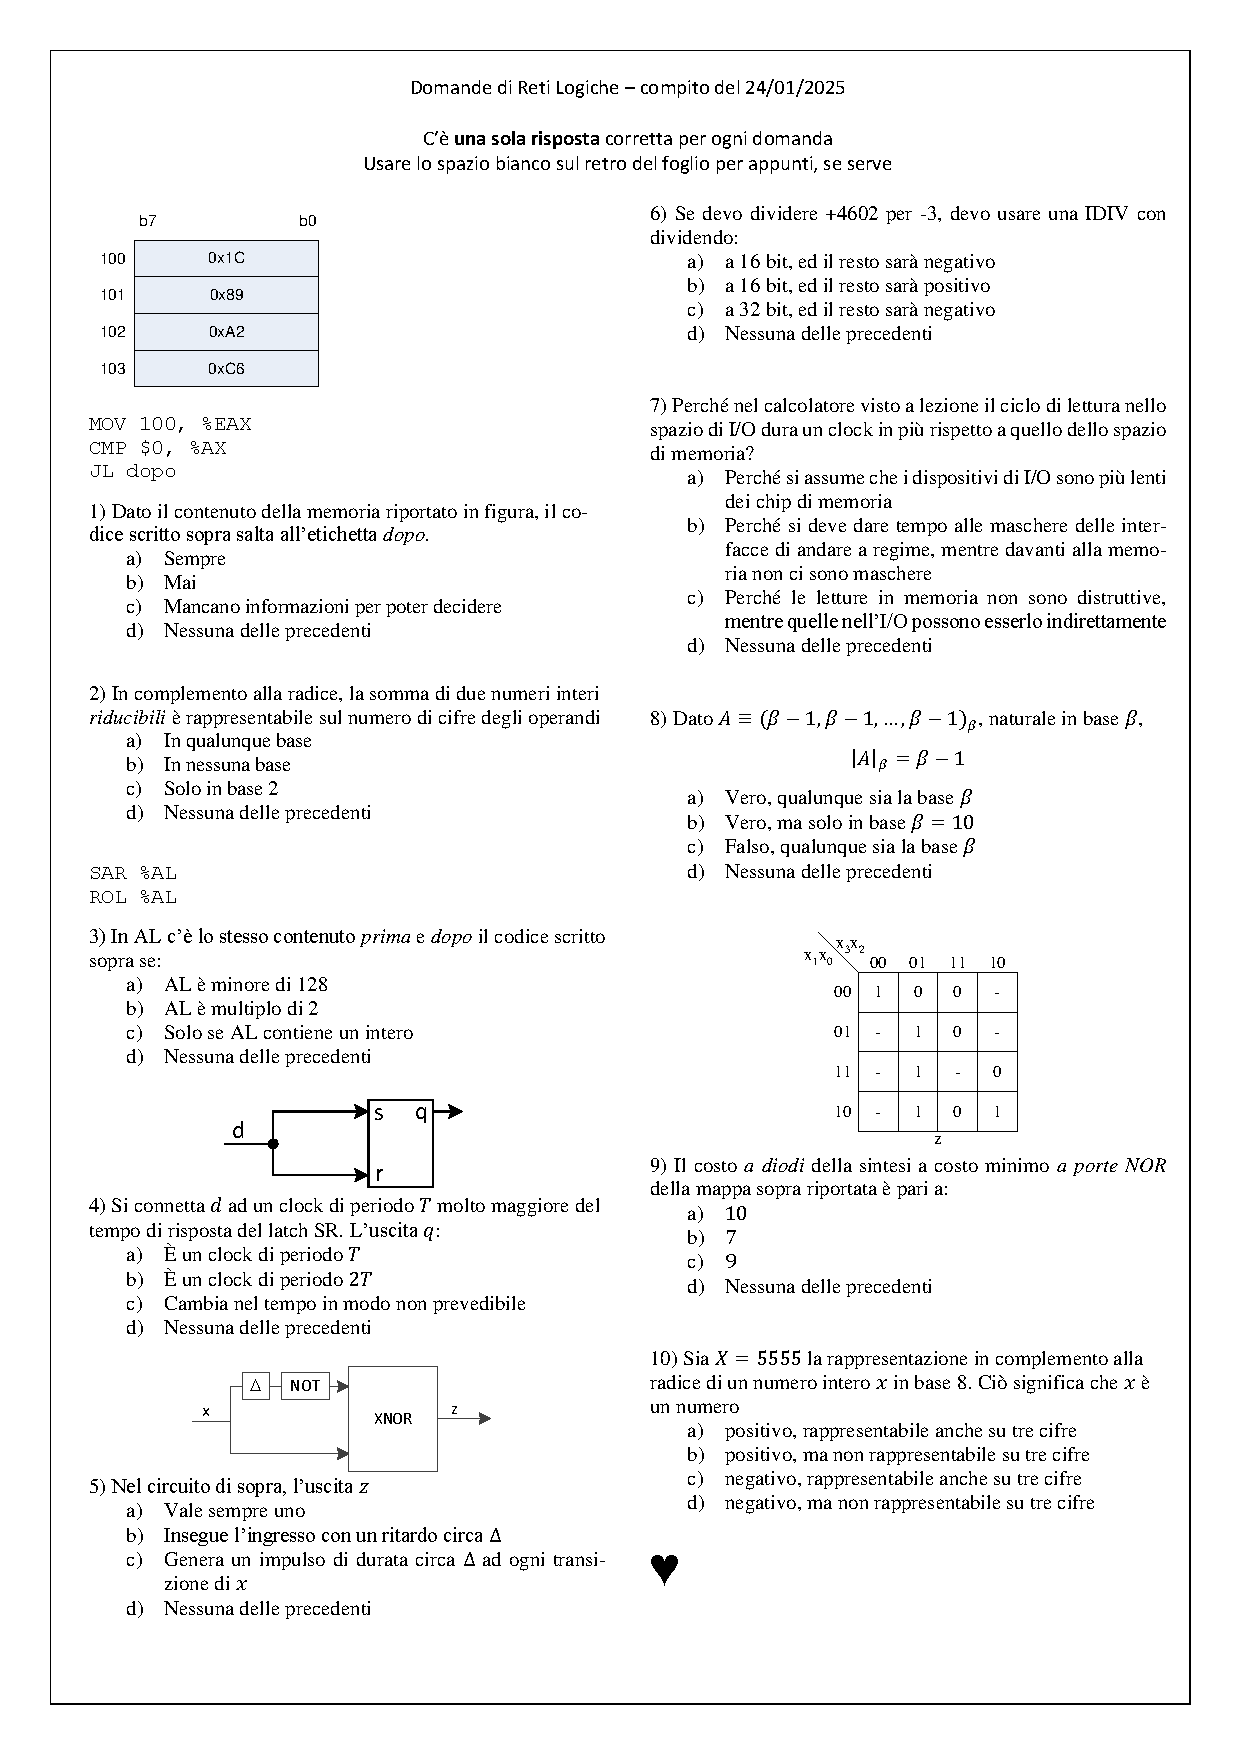
\includegraphics[width = \textwidth]{pretestImage/Domande RL 20250124.pdf}

\noindent\hspace*{-1.5cm}
    \begin{tabular}{|C{0.7cm}|C{8cm}|C{8cm}|}
        \hline
        \textbf{\#} & \textbf{High-level} & \textbf{Solution} \\
        
        \hline
        
        1 
        &
        I need to know how MOV moves data into registers $($ in what order $)$
        & 
        \begin{itemize}[label=\(\rightarrow\)]
            \item We're working in \textbf{little-edian} so the least significant byte is stored in the lowest address
            \item Smallest + i = smallest + i, iterated for each 9 bit memory address
        \end{itemize}   
        \\
        
        \hline


        2
        &
        Need to understand the conditions for a \textbf{riducibile} integer, and the arithmetic of riducibile numbers
        &
         \begin{itemize}[label=\(\rightarrow\)]
            \item Definition of a reducible integer in Anki 
            \item Worst case scenario is the addition between natural numbers, which works
            \item Given all the \textit{other bases} can be \textbf{represented} in base 2, if it works in base 2, it works in all 
        \end{itemize}   
        \\
        
        \hline

    \end{tabular}



\end{document}